\chapter{Desarrollo con tarjetas gráficas}

\section{Breve historia de la computación con GPUs}

Desde hace bastante tiempo se lleva usando las capacidades de las tarjetas gráficas para realizar computación. Concretamente se han utilizado para la realización de efectos sobre texturas y polígonos con la tecnología denominada shaders. Estos shaders son pequeños programas que transforman la forma de verse los puntos o como se transforman los polígonos y que se han estado ejecutando en las GPUs para mejorar su rendimiento.

A partir de esta tecnología y tras numerosas especulaciones sobre las capacidades de las tarjetas gráficas para realizar cálculos más genéricos, las compañías empezaron a abrir sus sistemas para permitir cargar códigos orientados a cualquier tipo de cálculo matemático.

Los primeros productoos con este tipo de tecnología provinieron de BionicFX y fueron presentados a principios de 2005 \cite{website:extremetech_gpu_audio}. En este caso se hacía uso de gráficas con GPU NVIDIA para procesador de audio. Para ello transformaba el sonido en datos gráficos y luego éstos se procesaban con los medios matemáticos de que disponía la GPU.

Más tarde, en el año 2006, la compañía AMD anuncia la comercialización de AMD Stream Processor \cite{website:amd_press_stream}, el primer sistema de cálculo basado en tarjetas gráficas. De este modo se empezó a comercializar el primer sistema que realmente permitía cargar código de usuario en la tarjeta para realizar cálculos que no estuviesen directamente relacionados con generación de imagen en 3D.

La compañía NVIDIA publica el 15 de febrero de 2007 la bibliotecas CUDA \cite{website:nvidia_press_cuda} que permite usar sus tarjetas gráficas para cálculo y, además, comercializa la arquitectura Tesla que, como en el caso de ATI, es un sistema específico de cálculo basado en tarjetas gráficas.

En base a esta popularización del cómputo con tarjetas gráficas y por  su utilizad gran utilidad para todo tipo de procesos (especialmente aquellos destinados a multimedia e investigación), Apple publica un borrador de OpenCl (Open Computing Language) y posteriormente éste es pasado a control de Khronos Group \cite{website:khronos_press_opencl}. OpenCl es  el primer estándar creado específicamente para cómputo distribuido, orientado principalmente a GPUs, y que ofrece una interfaz común para todo tipo de tarjetas gráficas y otros sistemas de cálculo (como procesadores multinúcleo, FPGAs, procesadores CELL, etc.). Esta tecnología solo se incluye de serie en el sistema operativo Apple Mac OS X 10.6, pero fabricantes como ATI y NVIDIA proveen de controladores para otras plataformas.

El mecanismo más eficiente para aprovechar las capacidades de una tarjeta gráfica es utilizar la API del fabricante ya que éste está optimizado para aprovechar mejor la arquitectura. Esto supone que en casos en los que la eficiencia es algo absolutamente crítico sea mejor opción frente al uso de la biblioteca OpenCl.

Estos sistemas están teniendo mucha relevancia debido a su alto rendimiento, especialmente en aplicaciones científicas. Además, se han realizado avances en el desarrollo de aplicaciones específicas de ruptura de contraseñas.

En la actualidad la computación con tarjetas gráficas está empezando a utilizarse en todo tipo de cálculos, tanto para investigaciones científicas  como para herramientas de usuario como descompresores de vídeo y audio, filtros gráficos en herramientas de diseño o videojuegos. Todo esto gracias a las grandes capacidades de paralelización de cálculos de las GPUs como a la faciliad de realizar cálculos vectoriales de forma sencilla. Esto significa que es una tecnología apoyada por la industria y que se va a disponer de soporte y documentación para realizar desarrollos con la misma.

Se puede comprobar, además, como en el año 2008 empezaron a surgir los primeros sistemas orientados a la seguridad informática que se apoyaban en el uso de tarjetas gráficas para realizar dicha función. Un ejemplo de esto lo tenemos en la herramienta de Elcomsoft publicada en octubre de 2008 \cite{website:elcomsoft_press} que hace uso de tarjetas gráficas para recuperar contraseñas.

\section{Introducción a CUDA}

Para desarrollar este proyecto se ha hecho uso de la tecnología CUDA de NVIDIA por varios motivos:
\begin{itemize}
	\item Las tarjetas gráficas NVIDIA están muy distribuidas y vienes de serie en la mayor parte de equipos informáticos de gama media/alta.
	\item El uso de un API específico ayuda a aprovechar mejor las características de la arquitectura frente a un API más general como pueda ser OpenCl.
	\item En el momento de realizar este proyecto se dispone de un sistema NVIDIA Tesla, por lo que CUDA se convierte en la solución ideal.
\end{itemize}

A la hora de desarrollar en una nueva arquitectura es importante conocer las características de la misma. Estas características pueden ir desde cómo se gestiona la memoria, qué instrucciones posee, etc.

En el caso concreto de la arquitectura CUDA hay que tener muy en cuenta la organización de la memoria (figura \ref{fig:memcuda}) ya que el buen uso de ésta influirá de forma muy significativa en el rendimiento de los programas. Esta arquitectura es la misma que la de las tarjetas gráficas y se puede representar como una pirámide de tiempos dependiendo del tipo de memoria a la que se vaya a acceder.

\begin{figure}
	\centering
	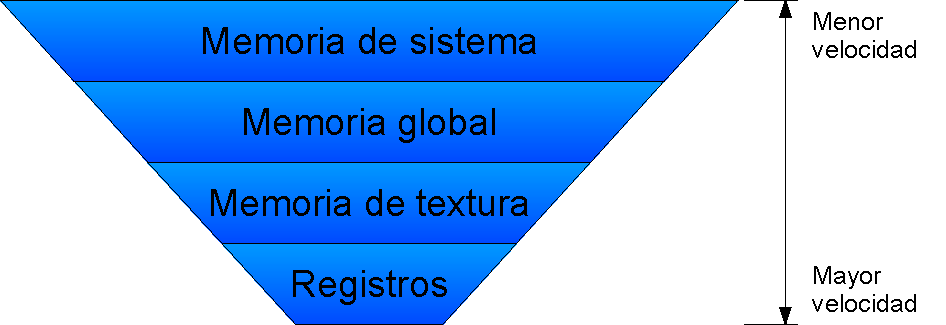
\includegraphics[width=0.7\textwidth]{images/MemoriaCuda.pdf}
	\caption{Jerarquía de memoria en CUDA}\label{fig:memcuda}
\end{figure}

Para el código CUDA la memoria del sistema es inaccesible por lo que solo puede hacer uso de la memoria que se encuentra en la propia unidad de cómputo (normalmente en la tarjeta gráfica). Esto supone que antes de realizar operaciones sobre memoria en CUDA hay que reservar la memoria e inicializarla desde el programa principal (la parte que no se encontrará en la GPU). Esta inicialización suele realizarse en tres tiempos. En un primer momento se preparan los datos que se pasarán a la GPU, seguidamente se reserva la memoria en la tarjeta gráfica y por último se copian los datos a la tarjeta gráfica para poder ser usados desde la parte que será ejecutada en la GPU.
Por otra parte es importante tener en cuenta que una vez se disponen de los datos sobre la memoria de la tarjeta gráfica es importante estudiar si conviene utilizarlos desde dicho punto o si es preferible realizar una copia a registros de procesador que serán mucho más rápidos. Hay que tener en cuenta que la tarjeta gráfica provee de una gran cantidad de registros (hasta 16.384 en el caso de las NVIDIA Tesla) para poder acelerar los cálculos por lo que hay que se deberá hacer uso de los mismos en la medida de lo posible para acelerar la velocidad de ejecución de los códigos que se alojen en la GPU.
Por norma general, siempre que se hace un código que vaya a ser alojado en una GPU se realizará el siguiente proceso (figura \ref{fig:procejecuda}):

\begin{itemize}
	\item Se copian los parámetros que se hallen en memoria global a registros, siempre que sea posible, para acceder a los mismos desde ahí. Esto es especialmente importante si el número de accesos va a ser elevado ya que de otra forma se estaría desperdiciando una gran cantidad de tiempo en realizar accesos a memoria.
	\item Una vez que ya se tiene la memoria iniciada se procede a realizar los cálculos oportunos.
	\item Finalmente se preparan los resultados para ser volcados a la memoria global de la tarjeta gráfica y que de este modo puedan ser leídos por la aplicación.
\end{itemize}
 

\begin{figure}
	\centering
	
\includegraphics[width=0.7\textwidth]{images/proc_ejec1.pdf}
	\caption{Proceso de ejecución de un algoritmo en CUDA}\label{fig:procejecuda}
\end{figure}

Además de todo lo dicho, CUDA ofrece dos formas distintas para realizar el desarrollo. En la primera forma, la más sencilla, CUDA se encarga de realizar las llamadas al código que se alojará en la GPU de forma transparente de tal forma que no tendremos que preocuparnos de configurar muchos de los parámetros de los que dispone el sistema. Este mecanismo es muy útil y permite un desarrollo rápido de funciones así. Por otro lado estaría el sistema completo con el que debe utilizarse la API de CUDA y que permite un nivel más alto de granularidad. Con este sistema nosotros deberemos de realizar a mano la carga del código en la GPU, seleccionar la GPU de todas las posibles, etc.

\section{Instalación del entorno}

Una vez que se conoce como es la arquitectura, será necesario instalar el entorno CUDA en el sistema para poder utilizarlo. NVIDIA nos provee de 3 partes distintas:

\begin{itemize}
	\item El controlador gráfico con soporte de CUDA que es necesario para poder aprovechar las capacidades de cómputo de la tarjeta gráfica.
	\item El SDK que contiene todas la bibliotecas necesarias para poder desarrollar aplicaciones con soporte de ejecución en GPU.
	\item El Toolkit con las herramientas necesarias para generar los programas (como nvcc, el compilador de código CUDA) además de bibliotecas de alto nivel como BLAS y aceleración de FFT (transformada rápida de Fourier).
\end{itemize}

En la web de NVIDIA recomiendan que se instalen los componentes en el mismo orden en el que aparecen en el listado anterior.

A la hora de realizar la instalación de CUDA es importante tener en cuenta la plataforma (Windows, MacOS X, GNU/Linux) y las versiones. Para el desarrollo del presente proyecto fin de carrera se ha utilizado como equipo de desarrollo un sistema con Ubuntu 10.04 y el equipo de ejecución utiliza Debian GNU/Linux en su última versión estable.
